%%%%%%%%%%%%%%%%%%%%%%%%%%%%%%%%%%%%%%%%%
%%% WP01
%%%%%%%%%%%%%%%%%%%%%%%%%%%%%%%%%%%%%%%%%

\tsubsubsection{WP02 - Access to RI for Physics}

%%%%%%%%%%%%%%%%%%%%%%%%%%%%%%%%%%%%%%%%%
%%% Section content, please change!
%%%%%%%%%%%%%%%%%%%%%%%%%%%%%%%%%%%%%%%%%

\subsubsection*{Overview and Goals}

\begin{table}[H]
    \renewcommand{\arraystretch}{1.50}		
    \footnotesize   
    \begin{tabular}{*{3}{|p{0.10\textwidth}}|l|}
        \hline
        \rowcolor{mygray} \multicolumn{4}{|c|}{\textit{\color{white}Work Package Summary}} \\
        \hline
        \rowcolor{mylightergray} \textit{WP No.} & \cellcolor{white} 01 & \textit{Title of WP} & \cellcolor{white} WP Title \\
        \hline
        \rowcolor{mylightergray} \textit{Start} & \cellcolor{white} Mxx & \textit{End} & \cellcolor{white} Myy \\
        \hline
        \rowcolor{mylightergray} \multicolumn{4}{|p{0.978\textwidth}|}{\textit{Participating Organisations}} \\
        \hline
        \multicolumn{4}{|p{0.978\textwidth}|}{
            \hspace*{-0.75cm} 
            \begin{minipage}[t]{\textwidth}
    			\begin{itemize}
    			    \item WP Leader: Partner 1
    				\item Participants: Partner 2, Partner 3, Partner 4, Partner 5, Partner 6, Partner 7
    			\end{itemize} 
    			\vspace*{0.10em}
			\end{minipage}
        } \\
        \hline
    \end{tabular}
    \vspace{0.5em}\vfill
    \begin{tabular}{|p{0.978\textwidth}|}
        \hline
        \rowcolor{mylightergray} \textit{Goals} \\
        \hline
        \rowcolor{white} 
        \hspace*{-0.75cm} 
        \begin{minipage}[t]{\textwidth}
    		\begin{itemize}
    		    \item Goal 1
    			\item Goal 2
			    \item Goal 3
    		\end{itemize} 
    		\vspace*{0.10em}
		\end{minipage}        
        \\
        \hline
    \end{tabular}
    \vspace{0.5em}\vfill
    \begin{tabular}{|l|*{7}{>{\centering\arraybackslash}p{0.084\textwidth}|}}
        \hline    
        \rowcolor{mylightergray} \textit{Participant number} & \textit{1} & \textit{2} & \textit{3} & \textit{4} & \textit{5} & \textit{6} & \textit{7} \\
        \hline
        \rowcolor{white} \cellcolor{mylightergray}\textit{Participant short name} & Partner 1 & Partner 2 & Partner 3 & Partner 4 & Partner 5 & Partner 6 & Partner 7 \\
        \hline
        \rowcolor{white} \cellcolor{mylightergray}\textit{PM per participant} & xx & xx & xx & xx & xx & xx & xx \\
        \hline        
    \end{tabular}    
\end{table}

\subsubsection*{Status}

\todo{Briefly explain the status of the DoA.}

\subsubsection*{Progress per Task}
\subparagraph{Task 2.1: Stable Ion Beams (Month 02-2025)} \mbox{}

\todo{Briefly explain the progress of the task in context to the DoA.}

Period 2 has proven to be an extremely busy one for the Stable Ion Beam facilities of Task 2.1. All eight facilities (including several consortia) have supported multiple experiments with a very high level of success. A total of 80 projects were supported in P2. 

Whilst still performing the “traditional” forefront experiments in fundamental nuclear physics research, the program of science covered by the Stable Ion Beam facilities is very broad and multidisciplinary. Nuclear and accelerator-based techniques are being used to address to topics as far ranging as radiation shielding for lunar habitats (GSI-FAIR), radiation effects in 2D Nanostructures (GANIL), effects of heavy ion radiation on cells (GSI-FAIR and GANIL), thin film elemental characterisation for photovoltaic cells (CLEAR – IST), improved processes for purification of phosphogypsum (CLEAR – IST), assessment of the impact of dumping of radioactive materials in the Baltic Sea region (CLEAR – CNA) and analysis of air quality in the city of Naples (CLEAR – ATOMKI).

Of particular note are a number of experiments which highlight the importance to the community of having a large range of facilities of different scale, offering different ion beams and techniques, with efficient and flexible access available. Novel $^3$He and $^4$He targets, made by magnetron sputtering and trapped in a suitable substrate, were characterised at CLEAR-CNA and subsequently used in fundamental nuclear science experiments at other facilities. The $^4$He targets were used to study elastic alpha scattering on heavy nuclei relevant for nuclear astrophysics (ISOLDE IS698) and the $^3$He targets were to be used in the measurement of the lifetime of a subthreshold state in $^{15}$O using AGATA and SAURON at INFN-LNL. The $^{15}$O will be produced by neutron transfer to the $^3$He target from an $^{16}$O beam. At GANIL, experiments were made to assess the performance of thin, electrodeposited targets for future studies of Superheavy Elements (SHE) using high intensity ion beams. At CLEAR-IST, self-supporting $^{208}$Pb targets were characterised in order to reduce uncertainties in the analysis of Coulomb breakup experiments (for example $^6$He). CLEAR-ATOMKI characterised the tracking capability and sensitivity of detectors which will be used in a forthcoming experiment at n$\_$TOF neutron irradiation facility at CERN. At ALTO, an in-beam test was made to investigate the high-rate performance of the detectors and read-out chain which will form part of the G-NUMEN gamma-array demonstrator. In future, the NUMEN experiment will be focused on Nuclear Matrix Elements for neutrinoless double beta decay. 

At GANIL, there were two main themes in the studies carried out by the nuclear physics community – fission and nuclear structure in exotic systems. 

Complete isotopic fission yields from inverse kinematics transfer-induced fission in the thorium region were studied. Isotopic identification of fission fragments emitted from a number of fissioning systems produced by transfer reactions between a $^{232}$Th stable beam (new GANIL beam) and a carbon target was performed through the measurement of the target-like recoil in the Particle Identification Silicon Telescope Array (PISTA) detector.  The origin and competition between fission modes in the pre-actinides was studied, in the transitional case $^{192}$Po. The recent observation of a new asymmetric-fission “island”, located in the neutron-deficient pre-actinide region south-west of $^{208}$Pb, revealed the important role of additional, unforeseen, microscopically driven favoured proton configurations. While the transition from symmetric to asymmetric fission with increasing mass in actinides has been studied in detail, the transition from symmetric to asymmetric fission with decreasing mass in pre-actinides has not yet been mapped. The experiment aimed to collect such new data for neutron deficient pre-actinides, to track the transition from asymmetric to symmetric fission in the region and connect it to the actinide island. 

Nuclear structure in exotic systems was studied in several experiments. Spin-orbit splitting in the N = 19 isotones was studied with a view to providing essential input for theoretical models aiming at the description of the isospin dependence of the spin-orbit interaction and of the relative role of tensor and spin-orbit forces. The direct transfer reaction p($^{34}$Si,$^{33}$Si)d, with a secondary radioactive $^{34}$Si beam at an energy of 50 MeV/u, provided by LISE from the fragmentation of a $^{36}$S stable primary beam, impinging on a CH2 target was used. The detection set-up was composed of MUGAST + EXOGAM + Zero-Degree Detection (experiment e869). The cluster structure of the ground-state of light neutron-rich nuclei beyond alpha-clustering was investigated. Recent calculations predict that the light clusters d,t, $^3$He and $^4$He are all formed at approximately 1/10 of the nuclear saturation density, a condition typically reached in the surface region of nuclei. The $^{10}$Be(d,$^6$Li)$^6$He cross-section was measured in order to check the consistency between the transfer and knockout reaction approaches, as the $^{10}$Be(p,p$\alpha$) cross-section was previously measured at RIKEN. Extracted differential will further be compared with theoretical calculations making use of cluster wave functions calculated in a microscopic framework e.g. AMD (experiment e870).  The g-factor of the first 2$^+$ excited state in $^{22}$Ne was measured, of significant importance for two reasons: (i) the g-factor of this stable nucleus is of great theoretical interest, and (ii) although a high-precision value (~2$\%$) had been previously reported, it was called into question following measurements at ISOLDE on $^{28}$Mg. A highly accurate determination of g(2$^+$) in $^{22}$Ne will clarify the discrepancy and aid in the interpretation of data obtained for radioactive $^{28}$Mg from ISOLDE. Preliminary results already indicate that the previously reported high-precision value deviates by several sigma from our current observations (experiment e845).

At GSI/FAIR, the NUSTAR collaboration carried out three experiments during period 2. Currently a topic of investigation across the community, Multi Nucleon Transfer (MNT) reactions at the Coulomb barrier offer a promising route to produce unknown neutron-rich nuclei and possibly access the super heavy mass region. A new method combining a high-resolution TOF spectrometer (TOSCA) with a linear microcalorimeter (measuring kinetic energy) was tested. Precise $\Delta$E measurements behind a homogeneous solid absorber allow complete A and Z identification. A detector array of five units at 30$^{\circ}$ successfully implemented this technique (experiment G-22-00174). Continuing the high profile and high impact measurements of the structure of heavy elements, laser spectroscopy studies of californium, fermium, nobelium, and lawrencium continue efforts to probe nuclear structure near N=152 and Z=100. The established RADRIS technique and the high-resolution JetRIS method were used to expand level searches and investigate ground and isomeric states, such as the K-isomer in $^{254}$No thereby refining modern nuclear models (experiment G-22-00051). As astronomical observations of primordial deuterium reach ultra-high precision, reducing uncertainties in Big Bang Nucleosynthesis (BBN) becomes crucial. A study of electron screening effects, which currently remain inadequately understood and affect reaction rate calculations in astrophysical scenarios have been studied at CRYRING. This was enabled by measuring the D(D,n)$^3$He and D(D,p)$^3$H reactions at energies below 0.4 MeV/A using the CARME array (experiment G-22-00200/G-22-00201).

At the IFIN-HH Tandem Accelerator Complex, 22 experimental groups were supported and received beam time in period 2. Data analysis is ongoing for most groups, but several have already published or submitted their results for publication. Two experiments can be highlighted here. 
Octupole collectivity in $^{150}$Gd was studied at the ROSPHERE spectrometer in two complementary experiments aimed at measuring the lifetime of the 3$^-$ and 5$^-$ states using the recoil distance Doppler shift (RDDS) method and measuring the weak E3 transition branching ratios of these states populated in beta decay. A $^{13}$C beam incident on a thin $^{140}$Ce target was used to populated excited states in $^{150}$Gd in the RDDS experiment while a $^6$Li beam was used to produce radioactive $^{150}$Tb in order to study the beta decay to $^{150}$Gd. The combined experimental data showed increased B(E3) values, in particular the measured B(E3;3$^-$$\rightarrow$0$^+$)=45(5) W.u. being the highest and most precise octupole strength in the rare-earth region. State-of-the-art theoretical calculations performed using the Quasi-particle Random Phase Approximation not only reproduced the experimental B(E3) values in $^{150}$Gd but also the decreasing trend towards $^{146}$Gd. This work 
was published in Phys. Rev. Lett. and Phys. Rev. C.
Gamma-ray strength functions and nuclear level density in $^{112,114}$Sn were studied for the first time using the Oslo method. Thermodynamic properties and the structure of the pygmy dipole resonance were extracted and compared with existing data in the Sn isotopic chain. The results are compared with microscopic models implemented in the TALYS reaction code and the fully microscopic quasiparticle-phonon model for the underlying nuclear structure of the dipole strength in $^{112,114}$Sn. The quasiparticle-phonon model results show the importance of complex configurations to the low-energy dipole response in the pygmy dipole resonance energy region. The experimental data are further included in the cross-section and reaction rate calculations for the (n,$\gamma$) reaction of the p-process nuclei $^{112,114}$Sn showing a significant increase in reaction rates at high temperatures compared to existing nuclear databases. This work was submitted for publication in Phys. Rev. C. 

At JYFL, fourteen stable ion beam experiments were supported during the reporting period. The experiments were granted a total of 3096 hours of beam time access. Aside from one experiment which used the TOSCA two-arm time-of-flight spectrometer to study fission dynamics at the Large Scattering Chamber (NRO155), the remainder employed the recoil separators RITU and MARA to study various aspects of nuclear structure physics and reaction dynamics, in particular Multi-Nucleon Transfer reactions. The efficiency of performing campaigns at the separators, which can house the JUROGAM3 array of germanium detectors at their target positions , has been enhanced by the use of a gantry which allows the array to move from one separator to another within hours (see Fig.~\ref{fig:Jurogam3}). This removes the need to un-bias the detectors before moving the array, which previously resulted in a need to anneal the detectors to repair radiation damage. Such a procedure can take weeks-months. At MARA, themes have been studies of isospin symmetry in N=Z nuclei and measurements of nuclear excited state lifetimes using the APPA plunger device. Lifetimes were measured successfully in $^{94}$Rh, $^{86}$Mo and $^{62}$Ga. A further highlight from these studies was the first attempt to measure lifetimes in the N=Z nucleus $^{66}$As, which is an extremely challenging case with current state-of-the-art instrumentation. A first attempt was also made at in-beam spectroscopy of $^{114}$Ba, another very challenging case to the production cross section and difficulty to cleanly extract the channel of interest. At RITU, which is designed for studies of heavier nuclei, highlights included the measurement of lifetimes in $^{179}$Au and $^{192}$Pb (addressing questions in nuclear shape co-existence) and two experiments exploring the potential to use Multi-Nucleon Transfer reactions to study nuclei inaccessible by other means.

\begin{figure}[!h]
    \centering
    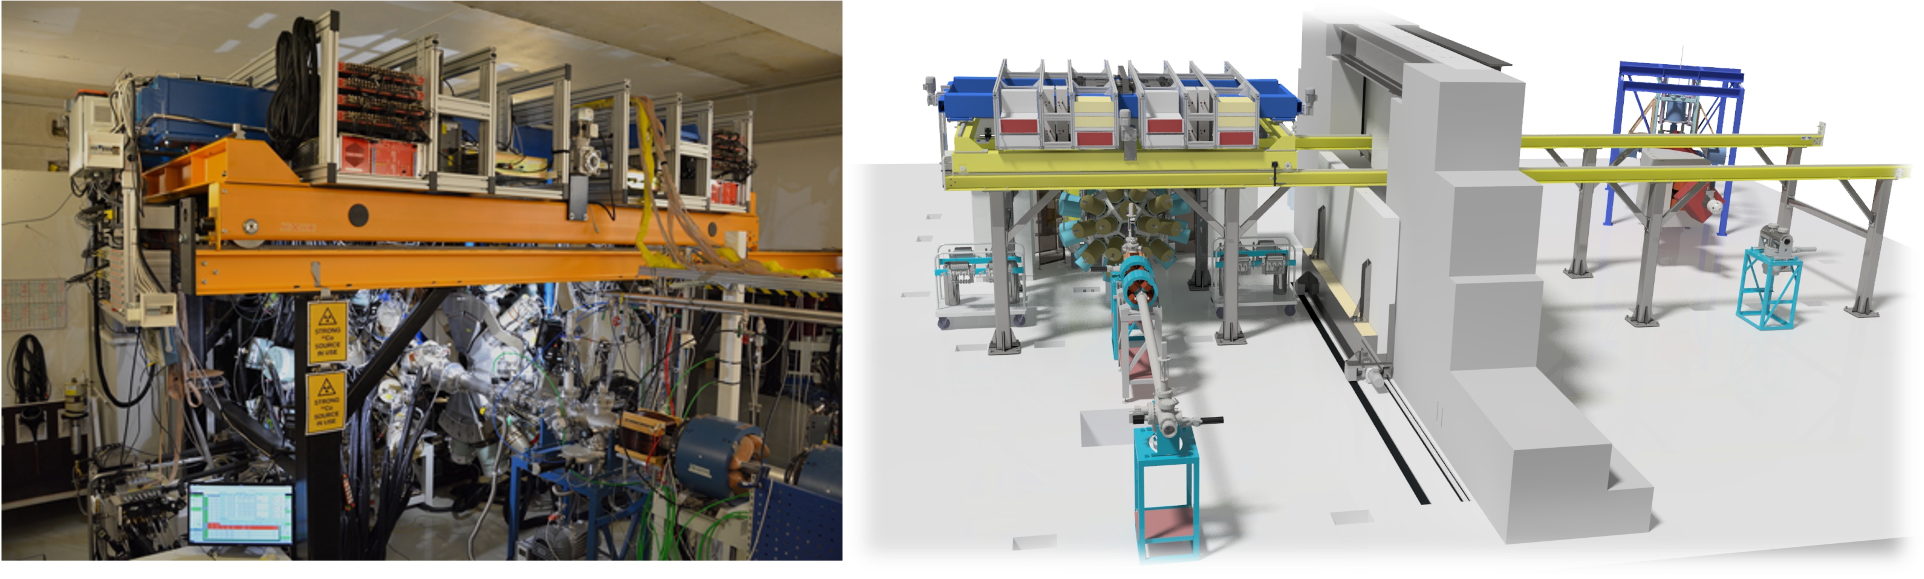
\includegraphics[width=1.0\linewidth]{graphics/Jurogam3.png}
    \caption{The JUROGAM3 array at the target position of the MARA recoil separator and the gantry system to allow rapid relocation of the array to the sister separator, RITU.}
    \label{fig:Jurogam3}
\end{figure}

At INFN-LNL, a total of ten experiments were supported during period 2. The experiments exploited the AGATA gamma-ray tracking array (see Fig.~\ref{fig:AGATA_LNL}) in various configurations with ancillary detectors. Using AGATA-SPIDER, a number of Coulomb excitation experiments were performed, for example to study the emergence of collectivity near $^{60}$Ni (experiment 23.008) and the interpretation of the structure of excited 0$^+$ states in $^{106}$Pd (experiment 23.054). AGATA-PRISMA was used, along with RDDS and DSAM techniques to measure lifetimes in $^{50-52}$Ca and $^{46-48}$Ar with a view to understanding shell evolution close to N=28 and Z=20 (experiment 22.81). The same devices were used to measure Multi-Nucleon Transfer (MNT) reactions. In the first experiment, the MNT reaction mechanism was investigated in the $^{130}$Te + $^{208}$Pb system (experiment 23.064), whilst in the second, MNT was used as a tool to populate and study the structure of nuclei in the island of inversion from the reactions of $^{26}$Mg beam on a $^{238}$U target (experiment 23.068). Other devices combined with AGATA for experiments were AGATA-SAURON, AGATA-EUCLIDES and AGATA-OSCAR. These show the versatility of the devices which can be modified for campaigns of experiments using different complementary techniques.

\begin{figure}[!h]
    \centering
    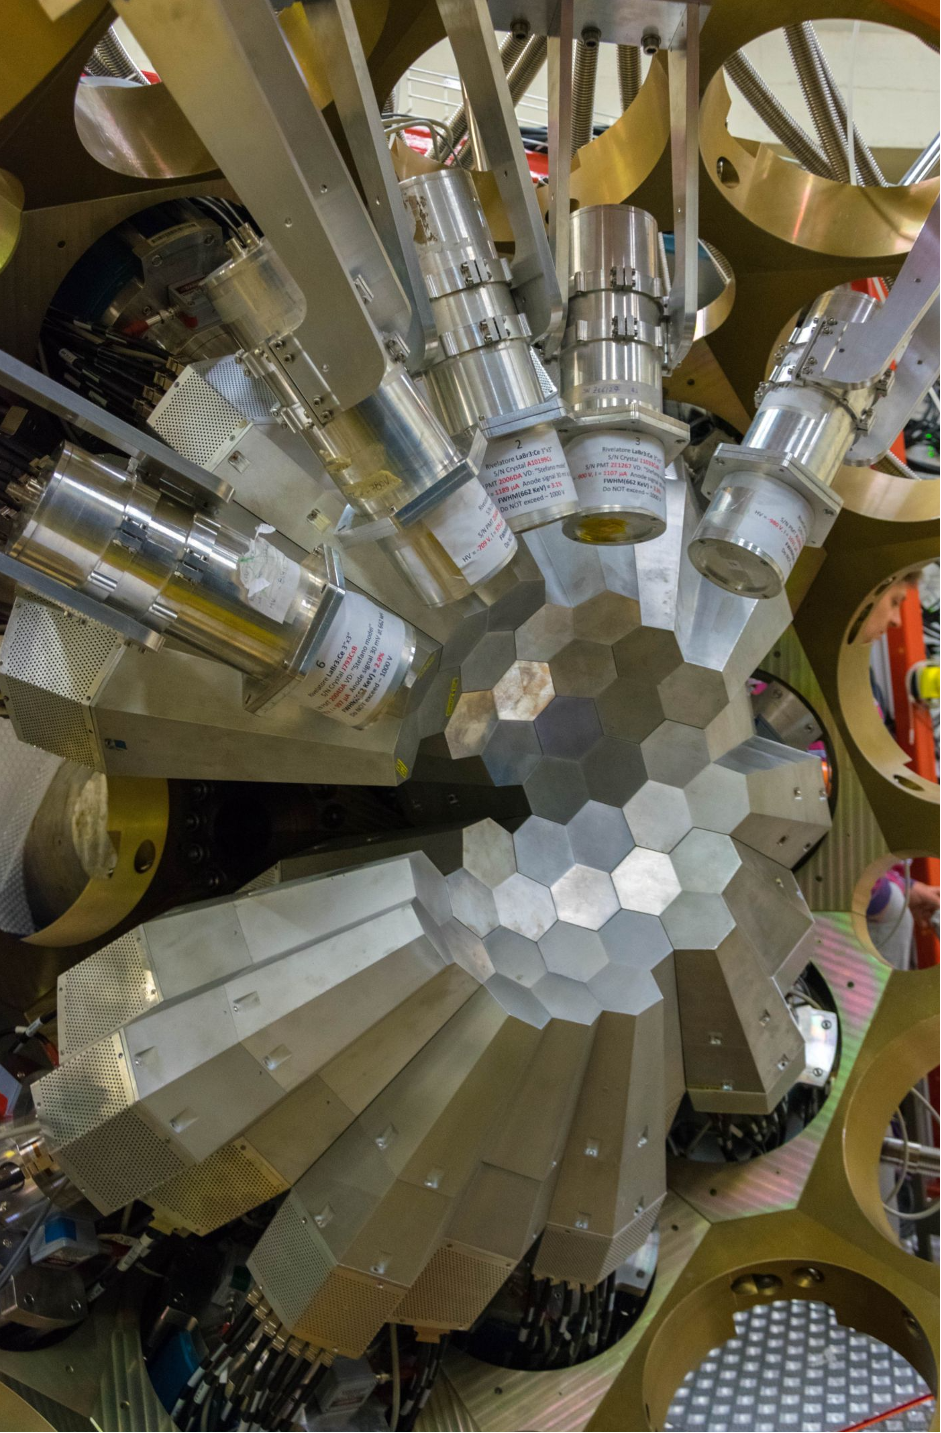
\includegraphics[width=0.6\linewidth]{graphics/AGATA_LNL.png}
    \caption{The AGATA gamma-ray tracking array installed at INFN-LNL.}
    \label{fig:AGATA_LNL}
\end{figure}

In period 2, two long (lasting few weekends each) experiments were performed at NLC-CCB (Krakow) with the use of high energy proton beams. 
The main objective of the first measurement (NLC$\_$CCB-004) was to study Pygmy Dipole Resonances (PDR) in stable nickel isotopes with proton beam and a high efficiency detector system to disentangle the paradigm of neutron skin oscillation and future application to nuclear astrophysics. The $^{58}$Ni and $^{62}$Ni nuclei were excited using inelastic scattering of 180 MeV protons. The high energy gamma rays emitted from the decay of excited nuclei were detected, using 4 high efficiency LaBr$_3$ scintillators and 26 PARIS phoswiches, in coincidence with scattered protons measured by KRATTA array. As a result, the $\gamma$-ray yield was measured and the PDR strength was determined for both isotopes, showing an increase for the higher neutron number. In addition, the polarisation for the low- and high-energy $\gamma$-ray region was determined. 
The aim of the second (NLC$\_$CCB-005) experiment was to study the decay of the M4 resonance state in 12C located at 19.5 MeV, by employing the 135-MeV proton inelastic scattering reaction. The objectives of the experiment were following: i) $^{12}$C(p,p') measurement at 135 MeV with thick, 150 mg/cm$^2$, $^{12}$C target for collecting the coincidence data between inelastically scattered protons, exciting the resonance, and gamma rays emitted from the decay products, ii) implementation and commissioning of the system of four Double-Sided Silicon Strip Detectors for light charged particles measurement, equipped with new, digital, read out, iii) $^{12}$C(p,p') measurement at 135 MeV with thin, 1 mg/cm$^2$, $^{12}$C target for recording the coincidences between inelastically scattered protons and light charged particles (protons, alphas) from the decay of the resonance. The experiment confirmed population of the resonance at energy 19.5 MeV in the $^{12}$C nucleus by the 135-MeV proton inelastic scattering reaction. From the energy of the scattered protons, the excitation energy spectrum of $^{12}$C was reconstructed. This spectrum is presented in the left panel of Fig.~\ref{fig:stretched_statest}, where the peak corresponding to the 19.5-MeV state is marked in red. In turn, right panel of Fig.~\ref{fig:stretched_statest} shows the coincidence matrix of the $^{12}$C excitation energy vs. gamma energy from preliminary, partial data analysis. The 4.4- and 15.1-MeV gamma transitions from the decays of states at these energies in $^{12}$C are clearly visible, as well as the 2.1-MeV line from $^{11}$B. Therefore, it is expected that a detailed analysis of the collected coincident and single data will allow to determine the intensity of the 19.5-MeV $stretched$ state's decay via the proton channel with the accompanying emission of a gamma ray from the daughter nucleus $^{11}$B. Furthermore, a commissioning of the digital acquisition chain for the system of four Double-Sided Silicon Strip Detectors was performed. 

\begin{figure}[!h]
    \centering
    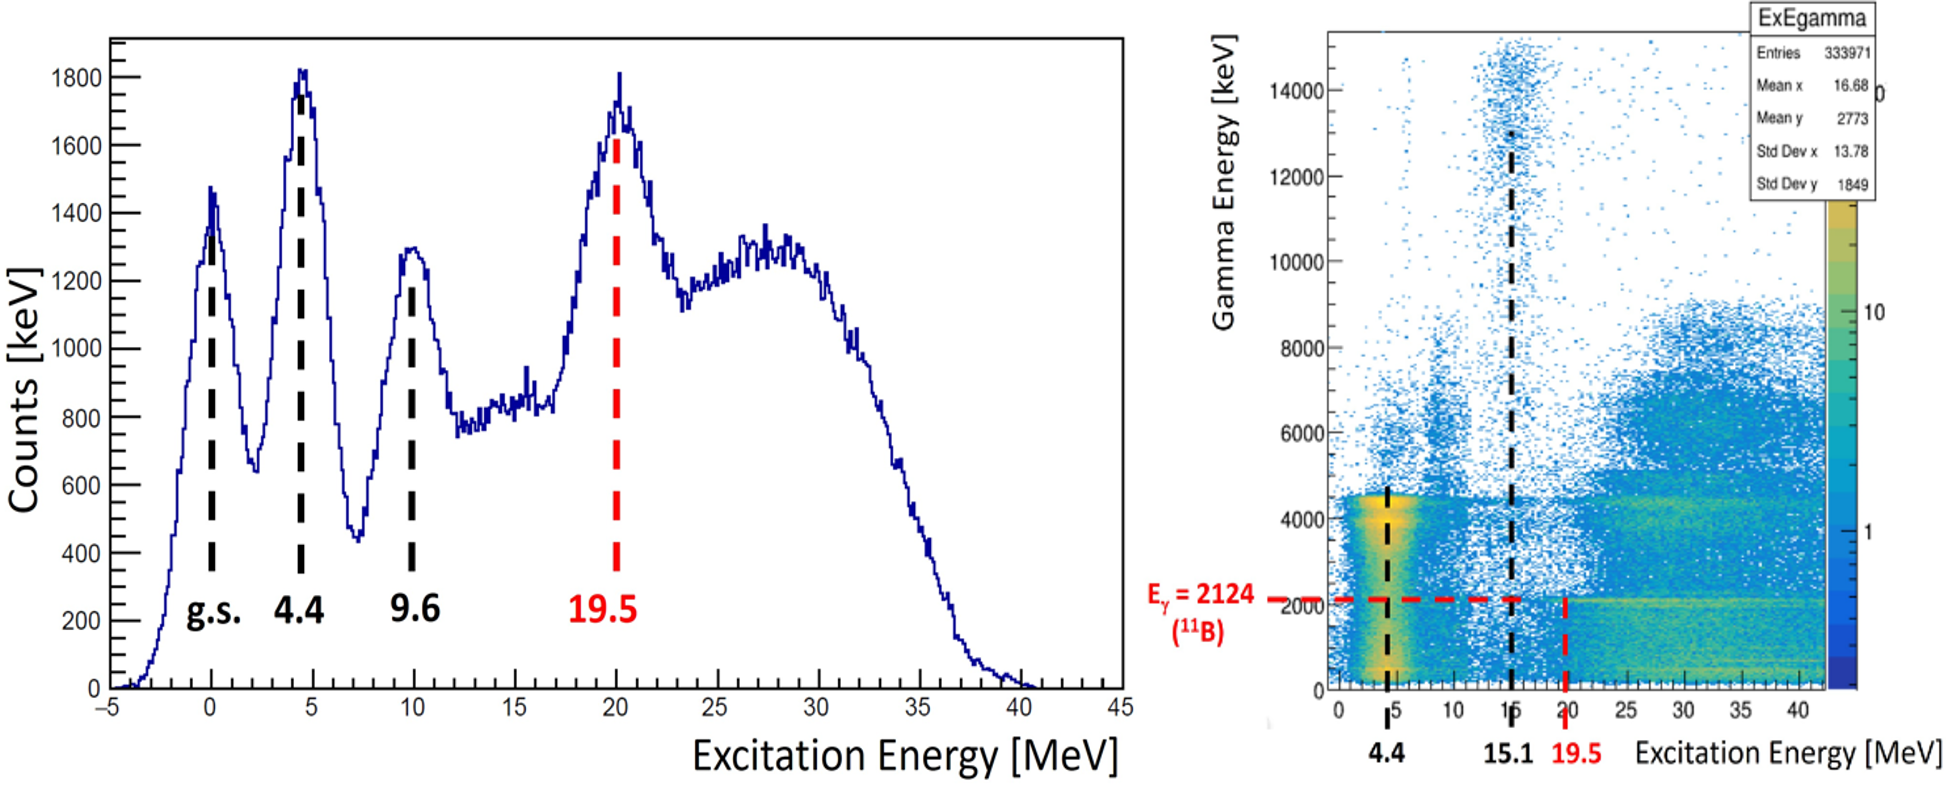
\includegraphics[width=1.0\linewidth]{graphics/stretched_states.png}
    \caption{Left: $^{12}$C excitation energy spectrum from proton singles. Right: Coincidence matrix of the $^{12}$C excitation energy and gamma energy.}
    \label{fig:stretched_statest}
\end{figure}

At NLC-SLCJ (Warsaw), six supported experiments were carried out in period 2.  
The EAGLE-NEDA-DIAMANT setup was employed in an experiment aimed at observing $\gamma$-ray radiation emitted from excited states of $^{57}$Cu, which has only one valence proton outside the doubly magic, self-conjugate N=Z=28, $^{56}$Ni core. The cross-section for the p2n reaction channel leading to $^{57}$Cu is expected to be in the 0.1 mb range, which, in relative terms, corresponds to about 3 × 10$^{-4}$ of the total fusion cross-section. The use of the NEDA and DIAMANT detectors was thus essential for selecting events of interest (experiment HIL-105). 
The N=Z=35 nucleus $^{70}$Br was studied to identify members of the T=1 isobaric analog states in $^{70}$Br with its even-even $^{70}$Se partner. The $^{70}$Br/$^{70}$Se isobar pair shows a unique behavior, with the Coulomb energy difference (CED) decreasing gradually with spin. Such an effect could be associated with significant shape changes with increasing angular momentum. However, the anomaly in the CED between the $^{70}$Br/$^{70}$Se isospin T=1 states remains a puzzle due to the lack of experimental data for $^{70}$Br. The goal of the experiment was to establish the position of the 6$^+$ and 8$^+$ states, which would help to understand the CED in the $^{70}$Br/$^{70}$Se isobar pair, as such a negative trend is not observed elsewhere (experiment HIL-115). 
Gamma-ray spectroscopic experiments were carried out to study excited states in $^{134}$Sm and to search for wobbling bands in $^{103}$Pd and $^{101}$Ru (experiments HIL-114 and HIL-126)
Reaction dynamics were investigated in an experiment dedicated to studying the influence of dissipation due to transfer channels on fusion barrier distributions. The systems studied were $^{20}$Ne+$^{92,94,95}$Mo at several beam energies. The masses of the products were identified using the Time-of-Flight (ToF) method. Preliminary results indicate that transfer leading to the masses A=19 and 16 were the main transfer channels in all three systems, but in the case of $^{95}$Mo, a neutron pick-up transfer (A=21) also occurred. The experiment should clarify the influence of such transfer channels on the different structures of the barrier distributions (experiment HIL-111).
The absolute transition strength between yrast levels in $^{172}$Os from level lifetimes measured with the recoil distance Doppler-shift (RDDS) technique and the Cologne plunger device, coupled to the EAGLE gamma-ray spectrometer was measured. Gamma-gamma coincidences were employed to rule out any contribution from unobserved side-feeding of the levels of interest, thus allowing for the unambiguous determination of the respective level lifetimes. A preliminary analysis of the data indicates that the lifetimes of the lowest yrast state in $^{172}$Os up to at least the 8$^+$ state can be determined (experiment HIL-109).


\subparagraph{Task 2.2: Radioactive Ion Beams (Month 02-2025)} \mbox{}

\todo{Briefly explain the progress of the task in context to the DoA.}

At GANIL-SPIRAL2 facility two projects received Transnational Access during EURO-LABS P2 focusing on Nuclear Physics investigations on light radioactive nuclei. One project, E837, focused on $^{12}$Be structure in the vicinity of different cluster thresholds, such as $^4$He, $^7$He, $^8$He by searching for narrow resonances using ACTAR-TPC detector. Second project, E864-22, focused at indirectly quantifying $^8$Li($\alpha$,n)$^{11}$B reaction. This reaction is involved in the nucleosynthesis from the early evolutionary stage of our universe, till the starting of r-process nucleosynthesis in supernovae, collapsars and neutron star mergers. The study has been performed by understanding the compound nucleus for the reaction, the neutron-rich $^{12}$B, with the help of the resonant elastic scattering reaction $^4$He($^8$Li,$\alpha$)$^8$Li.

The RI beams at GSI/FAIR are delivered to the nuclear and astrophysics community (NUSTAR). During EURO-LABS P2 period, fourteen user projects have been supported by Transnational Access. Within these experiments, different setups and parts of the facility were used as the experimental storage ring ESR, R3B experiment, DESPEC detector setup the FRS itself, the FRS Ion Catcher and EXPERT detector. Experiments using FRS recorded a comprehensive dataset for projectile-fragmentation products (Z = 82 to 89) from 238U on a Be target, providing essential data to refine fragmentation models and support future NUSTAR experiments. ESR has been used for investigating the rare double-gamma decay mode in 0$^+$$\rightarrow$0$^+$ transitions, this study measured isolated double-photon decays in $^{72}$Ge, and compared the two-photon decay in $^{98}$Zr and $^{98}$Mo to assess whether enhanced transition rates depend on nuclear structure and measures of de-excitation probabilities over a wide energy range in excited $^{238}$U and $^{239}$U. For the first time, simultaneous measurements of fission, gamma, and multi-neutron emission (up to three neutrons) were achieved in a storage ring setting. R3B setup has been used for commissioning of key detectors (CALIFA, Si-tracker FOOT, NeuLAND). Cross-section measurements for (p,pd) reactions on various carbon isotopes were performed indicating the presence of strongly correlated neutron-proton pairs, with quasi-deuteron behavior influencing nucleon “dressing” in the nuclear medium. DESPEC gathered spectroscopic data around N=126 shell closer, a critical region for r-process nucleosynthesis, where new level schemes and transition probabilities help benchmark models describing the interplay of single-particle orbitals and collective excitations in heavy nuclei relevant for the astrophysical sites. FRS Ion Catcher has been used in three different experiments. A proof-of-principle study using slowed-down uranium beams in a Cryogenic Stopping Cell demonstrated that multi-nucleon transfer (MNT) reactions can produce neutron-rich isotopes (A $\approx$ 160–250). MNT products were successfully extracted and identified with the MR-TOF mass spectrometer, paving the way for future RIB production at Super-FRS. Also focusing on exotic nuclei from Br to Rh, this study addresses issues such as isospin symmetry breaking, the Wigner effect, and unexpected mass discrepancies (e.g., $^{70}$Br). The FRS Ion Catcher, combined with a $^{107}$Ag fragmentation beam and SIS-18 accelerator mode, delivered precise mass measurements, essential for validating nuclear models and rp-process calculations. EXPERT detector using a $^9$C beam, the experiment probes Thomas-Ehrman shifts in mirror pairs (e.g., $^5$H-$^5$Be, $^6$H-$^5$B, $^7$H-$^7$C) and measures decay energies, widths, and half-lives (down to picoseconds) via multi-particle angular correlations. Upgraded high-rate tracking detectors have enabled high-statistics data collection, allowing for improved measurements of nuclear state widths and the identification of novel multi-proton decay mechanisms.

At JYFL total of six supported experiments were carried out using 888 hours of beam time access through Transnational Access during EURO-LABS P2. At IGISOL, by using a new beta detector made at NCNR (Swierk/Poland), trap-assisted decay spectroscopy of very neutron-rich Rh and Pd isotopes has been performed. An interesting experiment using a reaction of deuterons on $^{242}$Pu target(s), with the goal of producing both ground states and fission isomers in $^{240,242}$Am. Set of silicon detectors were installed in the switchyard, to be used for measuring alpha activity as well as fission fragments from the decay of the isomeric states. Operated in a “duty cycle mode”, with activity monitored in the switchyard as well as beam injected into the RF cooler, either for the MR-TOF or for JYFLTRAP. The latter allowed for separation of $^{242}$Am from the target $^{242}$Pu material. Half-lives were measured, total kinetic energy of the FFs as well as the excitation energy of $^{242f}$Am with the MR-TOF. Trap-assisted decay spectroscopy of fission fragments has been performed using a beta detector connected to a tape station and surrounded by a coaxial Ge and two large BeGe detectors. This setup allowed the collection of gamma-ray transitions with energy below 20 keV in A=115 isobars region. The I306 project focused on neutron-deficient Ag isotopes using collinear laser spectroscopy to provide a comprehensive data set that can be used to establish a precise and accurate reference quadrupole moment for the whole Ag chain. Combined with state-of-the-art atomic calculations the aim is to investigate the consistency of quadrupole moments deduced using atomic and solid-state crystal coupling constants. A second motivation was to determine the hyperfine anomaly in Ag, which reflects changes in the distribution of nuclear magnetization. 

At CERN/ISOLDE facility 64 projects received Transnational Access during EURO-LABS P2 focusing on Nuclear Physics investigations. Several experiments addressed very topical physics in nuclei around the $^{132}$Sn double shell closure. The $^{132}$Sn(d,p) reaction has underpinned the scientific cases of many different radioactive ion beam facilities, but only a single measurement existed from more than 15 years ago before a recent ISOLDE study. This experiment studied the reaction with around ten times the intensity of $^{132}$Sn, with a higher beam energy, and with a novel spectrometer giving much improved resolution. This revealed population of $all$ the valence single-neutron orbitals for the first time and their single-particle content has been deduced, establishing them all as carrying “full” single-particle strength. In parallel, $\beta$-delayed neutron decay studies at ISOLDE have also populated the 13/2$^+$ state, with even higher energy resolution. These data on a “simple”, but exotic, nuclear system will be very impactful as they can be used in shell-model calculations of wide regions of medium-mass nuclei. The collectivity of states in this region has also been probed in Coulomb-excitation measurements of $^{130}$Sn during this period. Also using post-accelerated beams, the reaction $^{61}$Ga(d,p) was used to populate the mirror nucleus of $^{62}$Zn, an important nucleus for the astrophysical rp-process. Mirror energy differences for high-spin states in the sdpf shell were probed in a measurement of $^{39}$K(d,p) and a search was made for rotational bands at high excitation with the same beam using a $^7$Be beam. On the low-energy side of the facility, studies of laser spectroscopy have continued with measurements across many chains of nuclides, including Mg, Ca, Sb, Lu, Tm, Au and Hg isotopes. The measurements of the hyperfine structure of neutron-rich Ca isotopes are of note, shedding light on the nature of exotic shell closures and performed using a new technique that allows measurements of isotopes produced at intensities as low as 1 ion per second. Similarly, laser spectroscopy of Mg isotopes, which probed the island of inversion, demonstrated another successful new technique where ions were trapped in a mass-resolving time-of-flight spectrometer, allowing improvement in sensitivity as the laser light can probe the same nucleus very many times. Work on radioactive molecules was continued by several experimental runs, including studies of electron photo-detachment from RaF$^-$. A high statistics run was performed on the WiSARD experiment looking at non-standard model currents in weak decays using $\beta$-delayed proton emitters. Nuclear techniques were employed to characterise a number of novel materials, which included perovskites that are potentially important for novel solar cells, vanadium-based materials that have important applications in batteries, indium-gallium nitride semi-conductors, quantum colour centers in diamond that may have application as q-bits, ferroic systems such as lithium niobate that is important in piezo-electrics, and other functional materials.

INL/LNS and ALTO had no Radioactive Ion Beams projects receiving Transnational Access during EURO-LABS P2.

\subparagraph{Task 2.3: Neutron Beams (Month 02-2025)} \mbox{}

\todo{"Briefly explain the progress of the task in the context to the DoA"}

At CERN's n\_TOF facility, seven projects were granted Transnational Access during the EURO-LABS P2 phase, focusing on various nuclear physics investigations. One project, INTC-P-665, explored new fission modes in lighter nuclear systems, particularly cerium isotopes around atomic number 60 (Neodymium). Three other projects concentrated on neutron capture cross-section measurements for isotopes of erbium and improving accuracy in existing data. INTC-P-872 specifically aimed to measure the $^{238}$U(n,$\gamma$) cross-section. Additionally, two projects investigated innovative techniques: INTC-P-831 measured neutron fluence using diamond detectors, and INTC-P-89

\begin{figure}[!h]
    \centering
    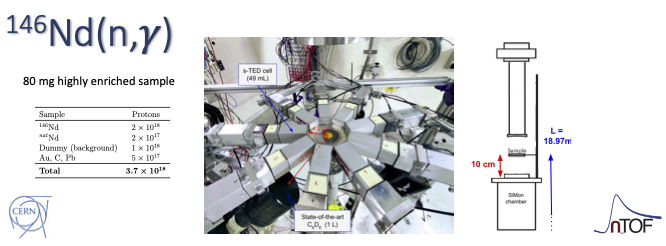
\includegraphics[width=1.0\linewidth]{graphics/n_TOF-146Nd.png}
    \caption{s-TED detector setup used at n\_TOF for for the $^{146}$Nd(n,$\gamma$) reaction cross section measurement, one of the seven TA experiments executed with the EURO-LABS project support.}
    \label{fig:n_TOF-146Nd}
\end{figure}

The CLEAR facility, involving IST Lisbon, ATOMKI Debrecen, and CNA Seville, conducted various experiments funded by EURO-LABS, focusing on environmental studies and isotopic analyses. Notable experiments included measuring actinides in Baltic seaweed, characterizing novel targets for astrophysics, and assessing the impact of radioactivity from nuclear facilities. 

At the ALTO facility, LICORNE projects refined fast neutron tomography techniques and studied radiation damage in LaBr$_{3}$ crystals under high neutron fluence, crucial for the NUMEN project. Lastly, at GANIL's NFS facility, two key experiments, E802 and E875, investigated gas production in chromium and copper, respectively. Both projects utilized advanced experimental setups to measure double-differential cross sections for neutron-induced reactions, contributing valuable data for future fusion plant simulations and nuclear reaction models. Overall, these initiatives highlight significant advancements in nuclear physics research and the importance of collaborative efforts across various facilities..

\subparagraph{Task 2.4: Theoretical Support (Month 02-2025)} \mbox{}

\todo{Briefly explain the progress of the task in context to the DoA.}

Theoretical support for experimental activities was enhanced in P2 following two subtasks. 

WP 2.4.1 enables in-person TA to the European Centre for Theoretical Studies in Nuclear Physics and Related Areas (ECT*, Trento). During P2, ECT* hosted 30 workshops and one Doctoral Training Program (DTP), following calls for proposals in the spring and summer of  2023 and 2024. Calls are made through the ECT* website (\url{https://www.ectstar.eu}) the extensive mailing list of ECT* associates. In addition, the ECT* Director and Scientific Board actively solicit proposals to ensure a balanced annual program.

Among the successful proposals, the Scientific Board, which serves as Selection Panel for EURO-LABS, selected for P2 10 workshops and the 2024 DTP. These activities covered microscopic optical potentials, strangeness reactions, nuclear theory and reactions for astrophysics, hadron tomography, the QCD phase diagram, the QCD plasma, neutrino interactions, electric dipole moments, high-power lasers, and machine learning. A highlight was the DTP, which introduced students from different backgrounds in nuclear physics and astrophysics to the current state of the art in the field of nuclear astrophysics, in particular new constraints on the equation of state of neutron-rich matter from nuclear theory, experiments, and observations, core-collapse supernovae as the birthplace of neutron stars, and mergers and gravitational waves as probes of the neutron-star interior. In this period, ECT* provided access to 133 EURO-LABS users. 

In addition, the Scientific Board has selected EURO-LABS activities for the remaining of 2025. They are workshops on ab initio nuclear theory, few-body physics, charge radii of light nuclei, neutron-capture reactions for astrophysics, information and statistics in nuclear theory and experiment, and lepton-flavor violation in nuclei. A highlight is a workshop in support of WP 2.4.2 activities. New calls in the spring and summer of 2025 will form the basis for the remaining EURO-LABS activities.

WP 2.4.2 provides access to theoretical tools through the virtual-access (VA) infrastructure Theo4Exp. It has been available since 1 February 2024 at \url{https://institucional.us.es/theo4exp}. Its opening to users has been posted in the EURO-LABS webpage and in social media, as well as distributed widely via mailing lists. The infrastructure consists of three installations: MeanField4Exp at IFJ PAN Cracow, Reaction4Exp at University of Sevilla, and Structure4Exp at University of Milano. The link to each installation can be easily found in the main webpage. User access to the installations is provided by the application \url{https://iam-eurolabs.ijclab.in2p3.fr/login}, which has been developed by WP5 of the present EURO-LABS project. This application ensures access to any researcher affiliated with a scientific institution via either eduGAIN (\url{https://edugain.org/}) or ORCID (\url{https://orcid.org/}).
An International Review Panel (IRP) meets every year to review and validate the progress made on the VA infrastructure and its three installations. The IRP is composed of P. Bednarczyk (IFJ-PAN, Chairperson), A. Moro-Mu\~noz (University of Seville), E. Vigezzi (INFN-Milano), K. Rusek (University of Warsaw), I.J. Thompson (Lawrence Livermore National Laboratory, LLNL), and A. Gargano (INFN-Napoli). Two meetings have been held in this period, on 20th September 2023 and 10th October 2024. A paper about Theo4Exp is scheduled to appear in the first 2025 issue of Nuclear Physics News (it is already accepted and at the proofreading stage). A hands-on workshop on Theo4Exp installations is scheduled for July 2025 at ECT* (\url{https://www.ectstar.eu/workshops/theory-service-for-the-low-energy-nuclear-physics-community-a-hands-on-workshop/}).

In P2 13 projects (virtual services) were offered and realized by 188 remote users. In total 1915 Access Units (counted as each started hour of active using of the virtual service) were provided. These numbers are almost twice higher as estimated for the whole duration of the project.

The activities for each installation comprised:

IFJ-PAN MeanField4Exp: A computer scientist, who was hired on 1 February 2023 for a period of 2 years, has worked on prepration of the installation website (\url{https://meanfield4exp.ifj.edu.pl/}).Several advanced nuclear structure theory computer programs developed earlier were adapted to the processors available in Cracow. In parallel, the interactive software allowing communication between external logged-in users and our VA infrastructure was tested. The whole system allows interactive communication with the computer programs as well as access to pre-calculated data sets according to user demand, with numerical results transferred in a professional output format (usually diagrams ready for publication). External users can select among the following options:
1. Calculation of single-nucleon energies as functions of nuclear deformation constructed within the mean-field-theory approach based the effective universal Hamiltonian, which depends on 12 parameters (6 for the protons and 6 for the neutrons) and provides a realistic, experiment-tested description of the single-nucleon spectra of all, nearly 3000 nuclei of the nuclear chart. The user can select the deformation-axis range and its multipolarity, as well as the standard Nilsson labelling of the curves, adapted to the publication standards.
2. Comparison of total nuclear potential energies calculated according to another literature standard, the Macroscopic-Microscopic Method (MMM). The user can plot several curves representing a selection of isotopes or isotones and allowing for a direct comparison of shape coexistence and competition within each nucleus. Both this and the previous option profit from the Inverse-Problem Theory, a branch of applied mathematics used to optimise the mean-field Hamiltonian.
3. Potential energy surfaces (2D maps) with user-chosen coordinate frames composed of multipole deformations ($a_{mn}$, $a_{m’n’}$). The default selection corresponds to the famous ($\beta$, $\gamma$)-shape parametrisation of Bohr, but numerous other choices are possible. This service is particularly well suited for identifying and examining nuclear shape competition, especially when interpreting experimental results.
4. Shape evolution with angular momentum based on macroscopic total nuclear energy surfaces especially adapted for the high-temperature description of shape evolution with spin. This option is practical and helpful for all those addressing shape transformations such as Jacobi and/or Poincare shape transitions, especially those relevant to nuclear giant dipole resonances.
5. Single-nucleon energies depending on nuclear frequency of rotation (cranking frequency), which helps the interpretation of results in terms of nuclear rotational properties within the so-called nuclear Cranking Model. Nearly completed extensions will allow the user to construct nuclear alignment plots as well as nuclear kinematic and dynamic moments. 
6. A graphical option to plot the shapes of nuclear surfaces (nuclear shapes) for a selected nuclear deformation.  By specifying the name of the point-group symmetry for the illustration of interest, two options allow the user to communicate with our system in terms of either the deformation multipolarities {$a_{mn}$} or the language of molecular symmetries.
These options will soon be supplemented by the possibilities of plotting a 3D representations of the nucleonic wave functions and of calculating reduced transition probabilities and lifetimes for both electric and magnetic transitions, which is particularly useful for the interpretation of the results of complex experiments. 

USE Reaction4Exp: A computer scientist, who was hired on 11 September 2023 for a period of 2 years, has worked on prepration of the main website (\url{https://institucional.us.es/theo4exp}) and  created the Reaction4Exp website (\url{https://reaction4exp.us.es}). In the main website she has included detailed information, photos, etc. The Reaction4Exp website includes the application for user access to the following calculations:
1. Coulomb breakup using the Equivalent Photon Model (EPM). The EPM code (developed by J.A. Lay Valera at University of Seville) calculates differential Coulomb breakup cross sections from external transition probabilities, as a function of both angle and energy. Multipolarities included are dipole and quadrupole for electric transitions and only dipole for magnetic transitions.
2. Elastic scattering using the Optical Model (OM). The OM calculation provides the angular distribution for the elastic scattering cross section of the reaction considered, at a given energy in the laboratory frame, if an optical potential is provided in order to describe the interaction between projectile and target. A classical calculation is also available (using a code developed by M. Gómez Ramos at University of Seville).
3. Inelastic scattering using the coupled-channel (CC) method and the distorted-wave Born approximation (DWBA). Results include the angular distribution for the cross section to each excited state and total reaction cross sections. 
4. Transfer reactions in DWBA. Defining the different partitions, the application provides the angular distribution for the transfer cross section from one partition to another, in which one particle is transferred from the projectile to the target or vice versa.
The code used for elastic, inelastic and transfer reactions is FRESCO, developed by I. J. Thompson, a close collaborator of the group at the University of Seville currently based at LLNL, USA.
The installation has been used already in various Master courses on nuclear reactions: Inter-university Master on Nuclear Reactions (Madrid, Barcelona, Granada, Salamanca and Sevilla), Erasmus Mundus Joint Master Degree on Nuclear Physics (Spain, France and Italy), and Master on Nuclear Structure and Astrophysics (Santiago de Compostela, Spain).

UMIL Structure4Exp: The person in charge of building the VA facility (\url{https://ns4exp.mi.infn.it/} was contracted between March 2023 and February 2024, with a partial overlap with the period under report. She has finished to implement and test the VA facility, which opened to the public before she left.  The installation hosted at the University of Milano offers two types of codes:
1. The first category includes codes for the calculation of basic spectroscopic properties of spherical nuclei throughout the mass table. Ground-state properties like masses and radii, as well as vibrational excited states, are provided. For each excited state, the codes give the transition strengths associated with isoscalar, isovector and electromagnetic operators. One can visualise how this strength is distributed among giant resonances and low-lying vibrational states. The two codes are self-consistent Hartree-Fock (HF) plus Random Phase Approximation (RPA), suitable for double-magic nuclei, or for nuclei with closed subshells both for neutrons and protons. The other code is based on HF+Bardeen-Cooper-Schrieffer (HF+BCS) plus Quasiparticle RPA (QRPA), and can be used for spherical, open-shell systems. Both codes employ a Skyrme-type effective forces.
2. The second type of code is the shell-model code KSHELL. This has been developed by N. Shimizu and collaborators at the Centre for Computational Sciences of the University of Tsukuba and its implementation has benefitted from the help of Giovanni Di Gregorio (Caserta University and INFN Napoli) and Angela Gargano (INFN Napoli). Calculations can be performed in different valence spaces, with a selection of appropriate interactions. Users can specify the energy levels to be determined, and the program provides energy, occupation numbers, main contributing configurations, and, if requested, E2 and M1 electromagnetic transition values. 
The installation has been visited by different scientists worldwide and it is envisioned to be used, partly, for a MSc course at the University of Milano.


\subparagraph{Task 2.5: Service Improvements (Month 02-2025)} \mbox{}

\todo{Briefly explain the progress of the task in context to the DoA.}

This task is divided into 5 different activities. A short summary of the lates progress is provided below.

WP2.5.1 Streamlined and remote access: 

a) In the Streamlined Access part of the subtask, the offer of facilities providing beam for nuclear physics research within the WP2 package has been presented in the form of a website (still under construction) \url{https://www.slcj.uw.edu.pl/en/tna-euro-labs/}. Each facility has its own subpage with a menu that provides easy access to specific information, such as: site details, list of available infrastructure and beams, beam time schedule, application deadlines, application submission deadlines and details, meeting dates, total number of access units in use and still available, access procedures, details of TNA support and the application process, and a list of publications. 

b) The Remote Access part of the subtask aims to provide improved remote access to EURO-LABS institutions (i.e., any kind of accessibility to experimental operation from outside of experimental areas for locals experts and external participants). The main goals are to minimise required access to experimental areas and minimise travel time for on-call experts, maximise external participation, and standardise generally-endorsed approaches and procedures. This subtask is divided into three main categories: i) the development of a user-friendly database to disseminate information on remote-access tools currently in use at EURO-LABS facilities, ii) the implementation of new/improved remote-access tools at EURO-LABS facilities, and iii) provide training opportunities to the community. The completion of part i) was reported in the official EURO-LABS project milestone M12 in February 2024. The database is fully operational (available here: \url{https://eurolabs-remote.gsi.de/}) and the collection of further information to expand the content is underway. A set of tools to provide remote control of the experimental irradiation setup are being implemented at the PARTREC facility, with the aim of minimising the amount of personnel needed on-site for guest research groups and/or paying customers of the PARTREC cyclotron.
To avoid potential security issues, users do not get direct access to the irradiation control system. Rather, they receive access (via VPN) to an interface PC connected to the (less privileged) internal network.
The interface PC can exchange text strings with the irradiation control PC via serial interface. A set of console commands in the form “DEVICE GET/SET [AMOUNT]” is provided, and a graphical interface is being worked on. Commands include, among others, beam on/off, energy setting via degrader, and beam shape via collimator.
A Python server running in the irradiation control PC parses the user’s input, and translates them into operations for the irradiation control system written in Labview, via the ActiveX interface. The server code will be open sourced in the near future.
Users also receive the live feedback from the irradiation room via the RTSP protocol. With the aim of advertising the "Remote Handling" database, a half-day workshop has been organised as a satellite meeting to the "VIIth Topical Workshop on Modern Aspects in Nuclear Physics" conference on Feb. 4th, held in Bormio (Italy). 


WP2.5.2 Targets for high intense beams: A database containing information on the preparation and characteristics of the targets available at the participating institutions, as well as those newly developed as part of this subtask has been completed. In particular, with the post-docs hired with EUROLABS funds at INFN-LNS and at GANIL, we collected information on the produced targets, their characteristics and manufacturing techniques from the collaborating institutions and the literature. The first version of this database is now ready and will be made public in the coming months via a user-friendly application.

WP2.5.3 Biomedical application (FLASH@EURO-LABS): Air-filled Farmer-type ionization chambers are widely used as standard detectors for absolute dosimetry in clinical settings. However, under Ultra-High-Dose-Rate (UHDR) conditions, these chambers experience significant recombination effects, resulting in high uncertainties in dose measurements.
The progress in this task was in 3 different topics: 1. Development and Benchmarking of a Numerical Model for Farmer-Type Ionization Chambers (cf. Fig.~\ref{fig:FLASH1}); 2. Application of the Developed Numerical Model: Evaluating the Reliability of the TM31023 Detector for Carbon Ion FLASH Applications; 3. Improvement of Dosimetry Uncertainty at Clinical Facilities.

\begin{figure}[!h]
    \centering
    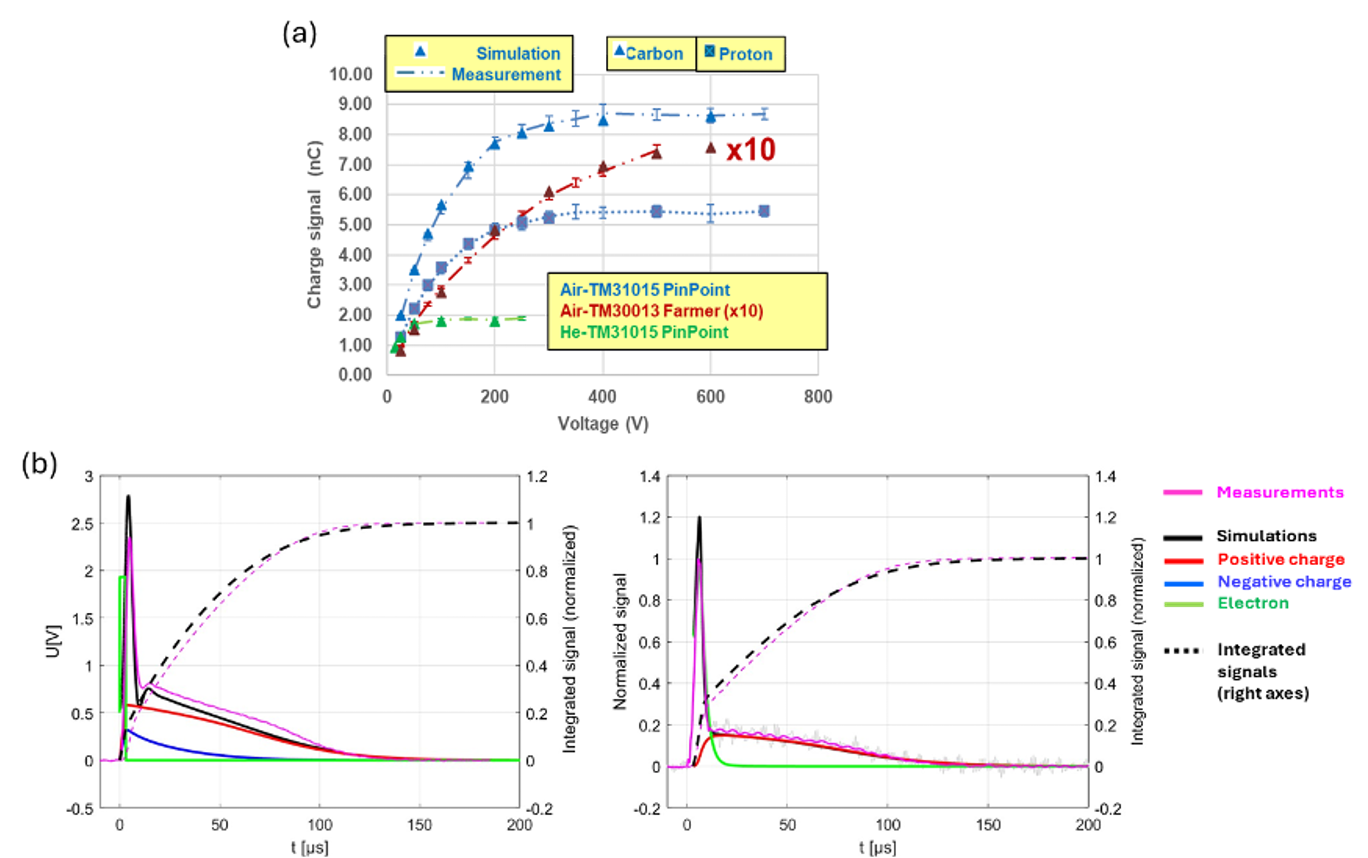
\includegraphics[width=1.0\linewidth]{graphics/FLASH1.png}
    \caption{Comparison of simulation and experimental data for FLASH dosimetry:
(a) Saturation curves of 3 different ionization chambers irradiated with protons at ultra-high dose rate at HIT in Heildeberg. (b) Time-resolved signals of the ionization chamber, whose integral corresponds to the charge collected by the electrometer, measured using a pulsed LINAC at Universitätsklinikum Gießen und Marburg (UKGM) at ultra-high dose rate. The signals from air-filled and nitrogen-filled Farmer chambers exhibit distinct differences in shape. This variation arises from the absence of electronegative molecules, such as oxygen, in the nitrogen-filled chamber, which prevents electron attachment.
}
    \label{fig:FLASH1}
\end{figure}

WP2.5.4 Improving Ion Beam services in variety and stability (ERIBS): The project has been divided into two separate parts to achieve the objectives. Part 1 focuses on extending the ion beam selection and intensities to allow new projectile-target combinations and/or to make low-cross section reaction studies possible. Part 2 focuses on developing online beam monitoring to maintain the requested beam intensity. In Part 1 the main progress was in the MIVOC service and technology transfer. In Part 2 progress was done in optical emission spectroscopy and online beam intensity monitoring.

WP2.5.5 Optimal employment of travelling gamma detectors (INTRANS): The INTRANS (Instrumentation and Training for Nuclear Spectroscopy and Reaction Dynamics) subtask has organized and/or sponsored a series of events since September 2023, including: Two AGATA Analysis workshops; InTraNS Workshop; Gamma Detectors Hands-on Training on operation, test and repair of Hyper Pure Ge Detectors; InTraNS Training Workshop on Coulomb Excitation.



\subsubsection*{Main Results and Achievements}

\todo{Briefly summarise the main results and achievements of the DoA in context of the DoA.}

In task 2.1, a number of the highlights from period 2 were referred to above, with the majority of groups now carrying out analysis on the data sets obtained. It is certain that in coming years a large number of publications and other outputs will result. Here we choose to select one scientific highlight which emphasises the complementarity of the facilities. 
The question of the properties of the E1 strength below the Giant Dipole Resonance (GDR) is of paramount interest for the understanding of the nuclei, testing theoretical models and has important implications in astrophysics. A series of experiments addressing this question were conducted in the isotopic chain of Ni isotopes going from the N=Z $^{56}$Ni up to the exotic nucleus $^{66}$Ni, and from zero to finite temperature. The measurements were done in the two EURO-LABS facilities IFIN-HH (Bucharest)) and NLC-CCB (Krakow). In the first one, a fusion evaporation reaction mechanism was used to create exited nuclei that emitted high energy gamma rays during the de-excitation process registered and detected with a high efficient and high resolution 4$\pi$ array of Compton supressed scintillator and light charged particle detectors.  For the very first time the extra yield below the GDR was observed at finite temperature in different Ni isotopes. In the second experiment, a complementary measurement by the same experimental group was carried out using inelastic proton scattering on stable nickel isotopes with the aim to investigate, for the first time in Ni isotopes, the low-energy part of the dipole response below and also above the neutron threshold at zero temperature. The experiment used a particle detector array as well as high efficiency scintillators detectors from the PARIS array to measure high-energy gamma rays and disentangle their polarity. The preliminary results are shown in Fig.~\ref{fig:Wieland}.

\begin{figure}[!h]
    \centering
    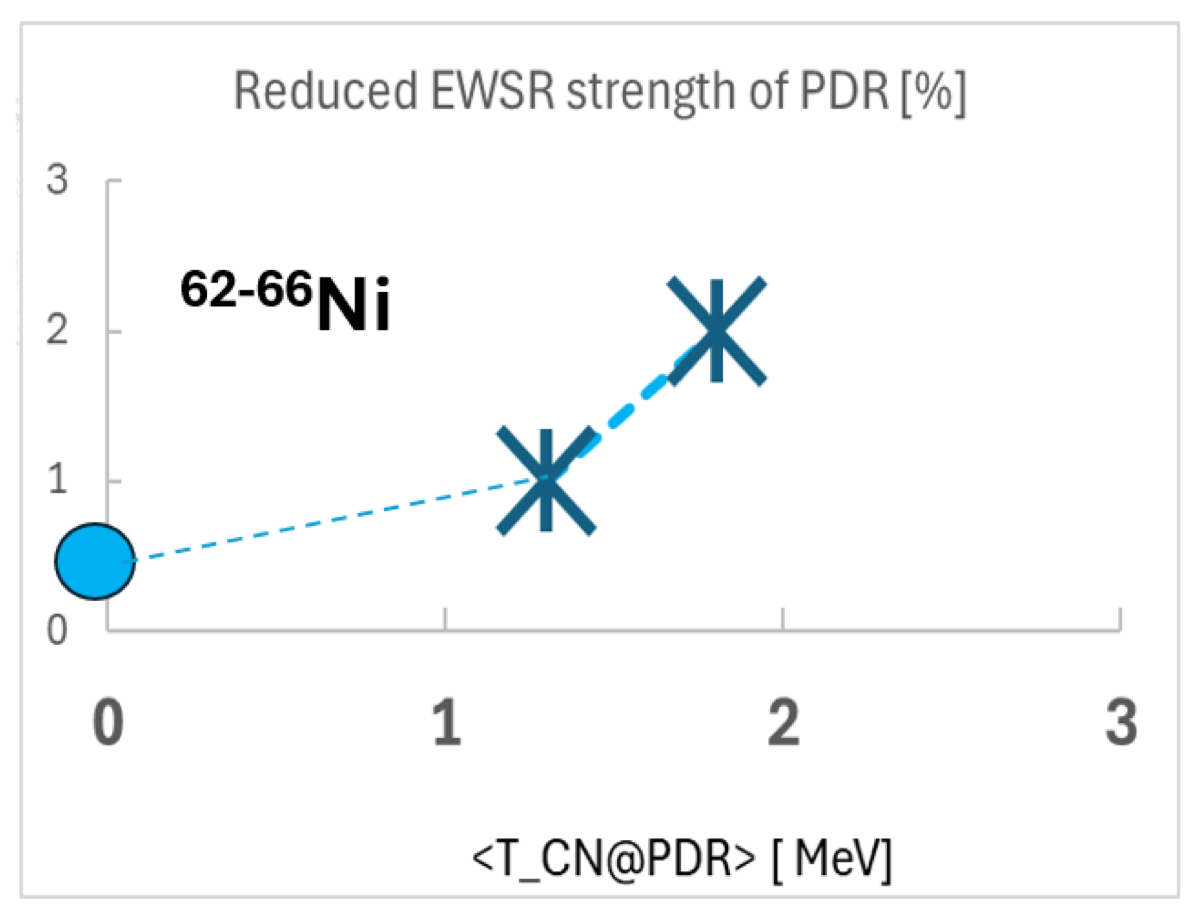
\includegraphics[width=0.6\linewidth]{graphics/Wieland.png}
    \caption{Combined preliminary results of the experiments done at CCB (circle) and IFIN (crosses). The plot shows the extra yield below the GDR for different Ni isotopes in function of the nuclear temperature.
}
    \label{fig:Wieland}
\end{figure}

Main achievements in the Task 2.2 were following:

Several experiments addressed very topical physics in nuclei around the $^{132}$Sn double shell closure at CERN/ISOLDE. The $^{132}$Sn(d,p) reaction has underpinned the scientific cases of many different radioactive ion beam facilities, but only a single measurement existed from more than 15 years ago before a recent ISOLDE study. This experiment studied the reaction with around ten times the intensity of $^{132}$Sn, with a higher beam energy, and with a novel spectrometer giving much improved resolution. This revealed population of all the valence single-neutron orbitals for the first time and their single-particle content has been deduced, establishing them all as carrying “full” single-particle strength (cf. Fig.~\ref{fig:ISOLDE_Highlight_1}). 

\begin{figure}[!h]
    \centering
    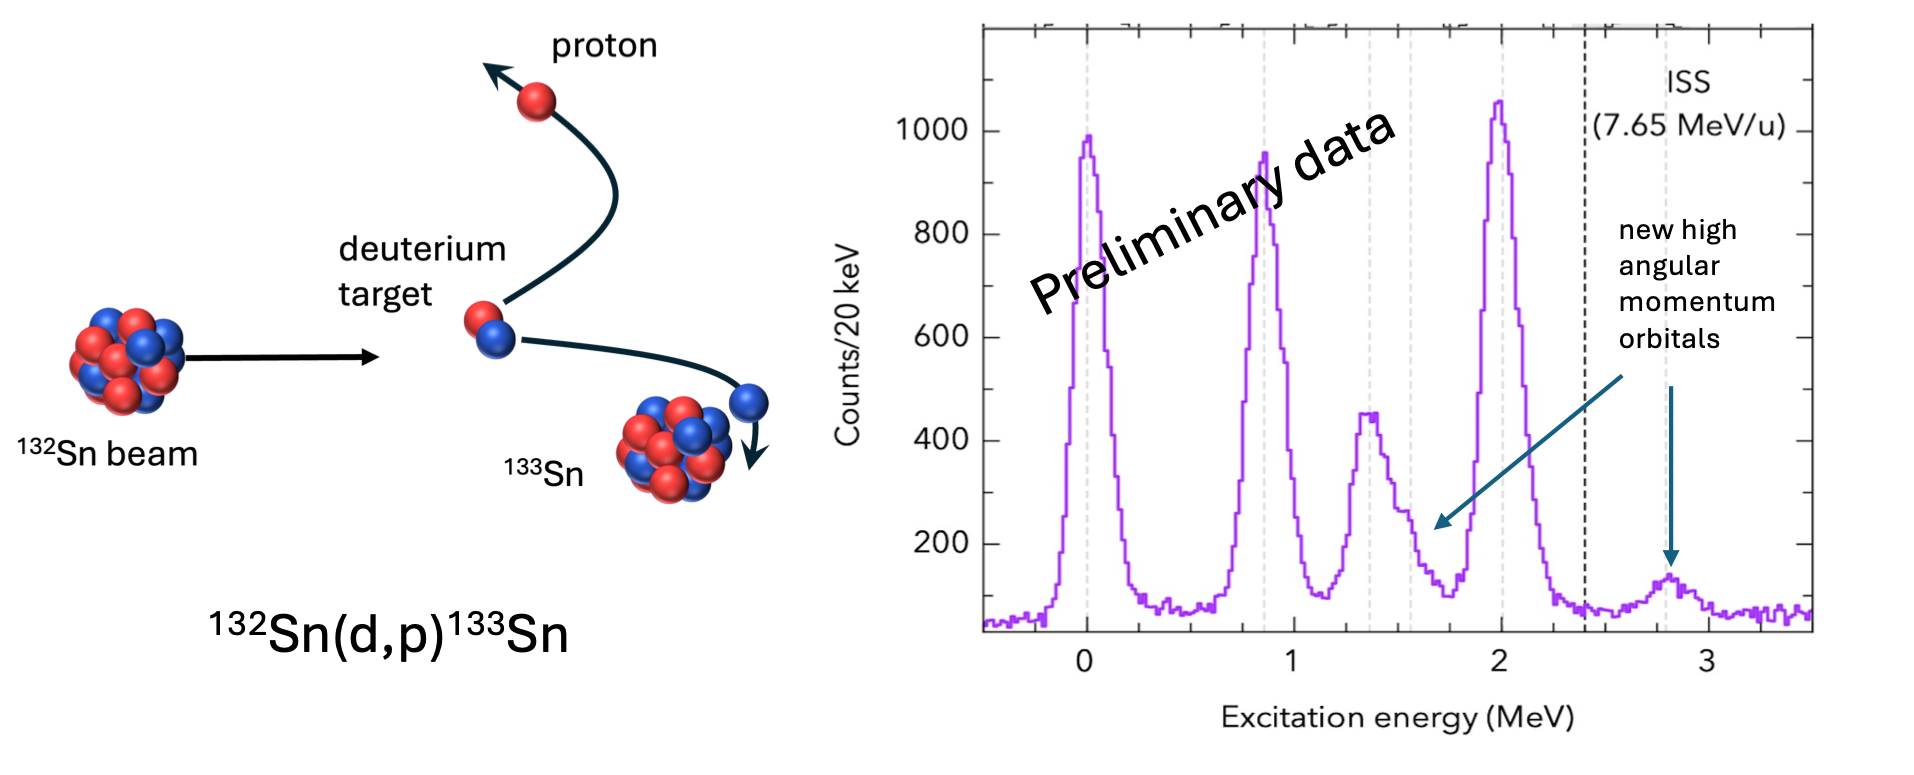
\includegraphics[width=0.9\linewidth]{graphics/ISOLDE_highlight_1.png}
    \caption{Left: A cartoon showing the mechanism for a direct (d,p) reaction.
Right: A preliminary excitation spectrum for $^{133}$Sn showing peaks corresponding to the single-neutron states outside the N=132 core.
}
    \label{fig:ISOLDE_Highlight_1}
\end{figure}

E837 project at GANIL/SPIRAL2 studied the $^{12}$Be structure in the vicinity of different cluster thresholds, such as $^4$He and $^8$He clusters using ACTAR-TPC detector (see Fig.~\ref{fig:2alpha_cluster}). 

\begin{figure}[!h]
    \centering
    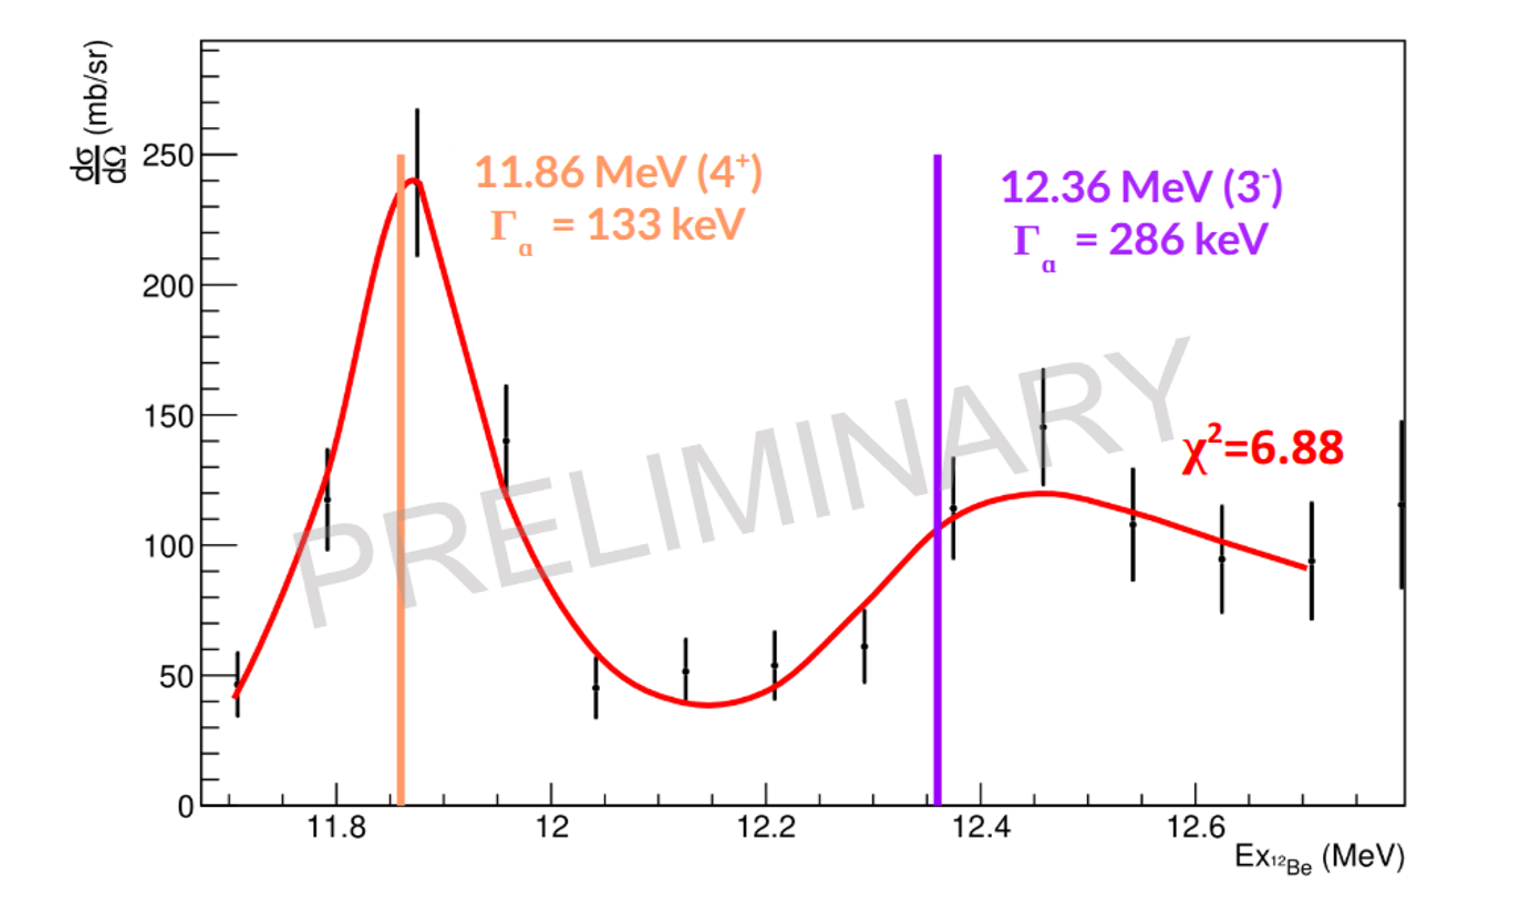
\includegraphics[width=0.7\linewidth]{graphics/2alpha_cluster.png}
    \caption{Two alpha cluster structure observed in $^{12}$Be by observing resonances in the resonance elastic scattering reaction $^4$He($^8$He,$\alpha$)$^8$He.The dark dots represents the experimental results, the red curve shows the quality of the theoretical decomposition of the results, while the violet and orange lines show the position of the cluster structure in $^{12}$Be.
}
    \label{fig:2alpha_cluster}
\end{figure}

I233 Project studied at JYFL joined a large collaboration from Spain (Valencia) and France (Subatech) at beta spectrometer after JYFLTRAP. This beta spectrometer has been used to directly measure the shape of the beta spectrum of several fission fragments. The motivation is connected to how well we understand the measured antineutrino spectrum from reactors.
This was an excellent beam time, following on from an earlier run in 2022. Expeirmental improvements meant that he yields as well as the overall transmission (between 25-60\%) from the switchyard to the beta spectrometer were excellent. In total, around 14 cases of interest (including references) were measured, with 1 TB of data collected. These data will be sufficient to satisfy the needs of a large number of doctoral researchers in the near future.


The main achievement in task 2.4 was the opening for external users, in February 2024, of the Virtual Access facility Theo4Exp. All three components of Theo4Exp have implemented theoretical tools for the evaluation of experimental data. MeanField4Exp at IFJ PAN Cracow now offers mean-field predictions for the evolution of nuclear shape with angular momentum, as well as the effects of deformation and shape on single-particle and potential energies. Reaction4Exp, now online at University of Sevilla, enables the calculation of Coulomb breakup, elastic and inelastic scattering, and transfer reactions. Structure4Exp at University of Milano provides properties like masses and radii for ground and excited nuclear states from self-consistent methods and the Shell Model. In addition, collaborations between theorists and experimentalists were stimulated by 10 workshops and an advanced school hosted by ECT* (Trento), covering various aspects of nuclear structure, reactions and astrophysics, as well as strong and weak interactions, fundamental symmetries, high-power lasers, and machine learning.

The main achievements in the task 2.5 period are: i) the delivery of new website in WP2.5.1; ii) a set-up for reduction and deposition in one-step of rare earth targets in WP2.5.2; iii) reduction of dosimetry uncertainty to <0.15\%, significantly improving accuracy, in proton therapy centers using Farmer-type ionizing chambers for FLASH in WP2.5.3; iv) the use of optical emission spectroscopy as a real-time monitoring to provide early indications about plasma instabilities in ERBIS; v) the success on the INTRANS workshop to the point that the INTRANS steering committee decided to hold an additional workshop towards the end of the EURO-LABS contract.





\subsubsection*{Deviations and Corrective Actions}

\todo{Briefly summarise any deviations and performed corrective actions of the DoA in context of the DoA.}

\subsubsection*{Milestones and Deliverables}

{\fontsize{9}{11}\selectfont
\begin{center}
  \begin{tabular}[t]{!{\color{mygray}\vrule}p{0.10\linewidth}!
  {\color{mygray}\vrule}p{0.60\linewidth}!
  {\color{mygray}\vrule}p{0.20\linewidth}!{\color{mygray}\vrule} } \hline
    \rowcolor{mycyan} & {\bf Title} & {\bf Status} \\ \hline
    \cellcolor{mycyan}{\bf MS8}: &Calls for proposals to be hosted at ECT*&  Achieved  \\ \hline
    \cellcolor{mycyan}{\bf MS10}: & Contracted personnel for Theo4Exp VA in place and first codes available for users in the virtual facility & Achieved \\ \hline    
    \cellcolor{mycyan}{\bf MS12}: & Completed database containing selected features of remote-access toolkit & Achieved \\ \hline 
    \cellcolor{mycyan}{\bf MS14}: & Reports on FLASH detectors for different facilities & Achieved \\ \hline 
    \cellcolor{mycyan}{\bf MS16}: & 	Organisation of hands-on workshops and training schools & Achieved \\ \hline 
  \end{tabular}
\end{center}
}

\subsubsection*{Project Meetings}

%  {\color{mygray}\vrule}p{0.40\linewidth}!







%%%%%%%%%%%%%%%%%%%%%%%%%%%%%%%%%%%%%%%%%


